%%%%%%%%%%%%%%%%%%%%%%%%%%%%%%%%%%%%%%%%%
%
% CMPT 435
% Lab Three
%
%%%%%%%%%%%%%%%%%%%%%%%%%%%%%%%%%%%%%%%%%

%%%%%%%%%%%%%%%%%%%%%%%%%%%%%%%%%%%%%%%%%
% Short Sectioned Assignment
% LaTeX Template
% Version 1.0 (5/5/12)
%
% This template has been downloaded from: http://www.LaTeXTemplates.com
% Original author: % Frits Wenneker (http://www.howtotex.com)
% License: CC BY-NC-SA 3.0 (http://creativecommons.org/licenses/by-nc-sa/3.0/)
% Modified by Alan G. Labouseur  - alan@labouseur.com, and Ryan Munger - ryan.munger1@marist.edu
%
%%%%%%%%%%%%%%%%%%%%%%%%%%%%%%%%%%%%%%%%%

%----------------------------------------------------------------------------------------
%	PACKAGES AND OTHER DOCUMENT CONFIGURATIONS
%----------------------------------------------------------------------------------------

\documentclass[letterpaper, 10pt]{article} 

\usepackage{tikz}
\usetikzlibrary{automata, positioning}
\usepackage[english]{babel} % English language/hyphenation
\usepackage{graphicx}
\usepackage[lined,linesnumbered,commentsnumbered]{algorithm2e}
\usepackage{listings}
\usepackage{float}
\usepackage{fancyhdr} % Custom headers and footers
\pagestyle{fancyplain} % Makes all pages in the document conform to the custom headers and footers
\usepackage{lastpage}
\usepackage{url}
\usepackage{xcolor}
\usepackage{titlesec}
\usepackage{ulem}

% Stolen from https://www.overleaf.com/learn/latex/Code_listing 
\definecolor{codegreen}{rgb}{0,0.6,0}
\definecolor{codegray}{rgb}{0.5,0.5,0.5}
\definecolor{codepurple}{rgb}{0.58,0,0.82}
\definecolor{backcolour}{rgb}{0.95,0.95,0.92}

\lstdefinestyle{mystyle}{
    backgroundcolor=\color{backcolour},   
    commentstyle=\color{codegreen},
    keywordstyle=\color{magenta},
    numberstyle=\tiny\color{codegray},
    stringstyle=\color{codepurple},
    basicstyle=\ttfamily\footnotesize,
    breakatwhitespace=false,         
    breaklines=true,                 
    captionpos=b,                    
    keepspaces=true,                 
    numbers=left,                    
    numbersep=5pt,                  
    showspaces=false,                
    showstringspaces=false,
    showtabs=false,                  
    tabsize=2
}
\lstset{style=mystyle, language=c++}


\fancyhead{} % No page header - if you want one, create it in the same way as the footers below
\fancyfoot[L]{} % Empty left footer
\fancyfoot[C]{page \thepage\ of \pageref{LastPage}} % Page numbering for center footer
\fancyfoot[R]{}

\renewcommand{\headrulewidth}{0pt} % Remove header underlines
\renewcommand{\footrulewidth}{0pt} % Remove footer underlines
\setlength{\headheight}{13.6pt} % Customize the height of the header

%----------------------------------------------------------------------------------------
%	TITLE SECTION
%----------------------------------------------------------------------------------------

\newcommand{\horrule}[1]{\rule{\linewidth}{#1}} % Create horizontal rule command with 1 argument of height

\title{	
   \normalfont \normalsize 
   \textsc{CMPT 432 - Spring 2025 - Dr. Labouseur} \\[10pt] % Header stuff.
   \horrule{0.5pt} \\[0.25cm] 	% Top horizontal rule
   \huge Lab 2 -- Finite Automata \\     	    % Assignment title
   \horrule{0.5pt} \\[0.25cm] 	% Bottom horizontal rule
}

\author{Ryan Munger \\ \normalsize Ryan.Munger1@marist.edu}

\date{\normalsize\today} 	% Today's date.

\begin{document}

\maketitle % Print the title

%----------------------------------------------------------------------------------------
%   CONTENT SECTION
%----------------------------------------------------------------------------------------

% - -- -  - -- -  - -- -  -
\section{Crafting a Compiler}
\subsection{Exercise 3.3 - Regular Expressions}
Create Regex for the following DFAs:
\begin{figure}[H]
    \centering
    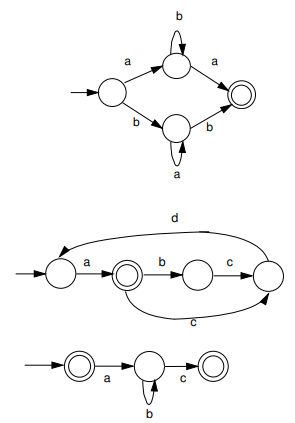
\includegraphics[width=.4\linewidth]{exercise3-3.png}
    \caption{DFAs for exercise 3.3}
    \label{fig:enter-label}
\end{figure}
\newpage
\noindent
\textbf{DFA \#1:} (ab*a)\textbar(ba*b) \\
\textbf{DFA \#2:} a((bcda)\textbar(cda))* \\
\textbf{DFA \#2:} $\epsilon$ \textbar (ab*c)  \\

\subsection{Exercise 3.4 - Deterministic Finite Automatas}
Write DFAs that recognize the tokens defined by the following regex: \\
On a side note, the TikZ and Automata packages are awesome! \\

1. $(a | (bc)* d)+$ \\
% DFA for (a|(bc)*d)+
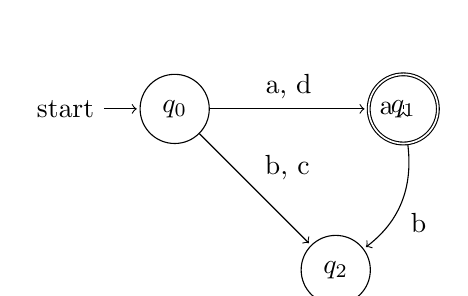
\begin{tikzpicture}[shorten >=1pt, node distance=2cm, auto]
    \node[state, initial] (q0) {$q_0$};
    \node[state, accepting] (q1) [right=of q0] {$q_1$};
    \node[state] (q2) [below right=of q0] {$q_2$};
    
    \path[->]
    (q0) edge node {a, d} (q1)
    (q0) edge node {b, c} (q2)
    (q1) edge[bend left] node {a} (q1)
    (q1) edge[bend left] node {b} (q2);
\end{tikzpicture} \\

2. $((0|1)(2|3)+)| 0011$ \\
% DFA for ((0|1)(2|3)+)|0011
\begin{tikzpicture}[shorten >=1pt, node distance=2cm, auto]
    \node[state, initial] (q0) {$q_0$};
    \node[state] (q1) [right=of q0] {$q_1$};
    \node[state] (q2) [right=of q1] {$q_2$};
    \node[state] (q3) [right=of q2] {$q_3$};
    \node[state, accepting] (q4) [right=of q3] {$q_4$};
    \node[state] (q5) [below=of q1] {$q_5$};
    \node[state, accepting] (q6) [right=of q5] {$q_6$};
    
    \path[->]
    (q0) edge node {0} (q1)
    (q0) edge node {1} (q5)
    (q1) edge node {0} (q2)
    (q1) edge node {2, 3} (q6)
    (q2) edge node {1} (q3)
    (q3) edge node {1} (q4)
    (q2) edge node {1} (q3)
    (q5) edge node {2, 3} (q6)
    (q6) edge[loop below] node {2,3} (q6);
\end{tikzpicture} \\
\newline

3. $(a \neg(a))*aaa$ \\
% DFA for (a Not(a))*aaa
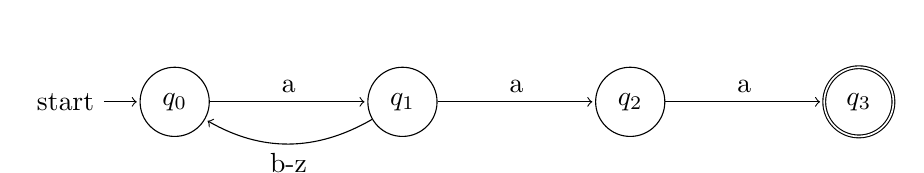
\begin{tikzpicture}[shorten >=1pt, node distance=2cm, auto]
    \node[state, initial] (q0) {$q_0$};
    \node[state] (q1) [right=of q0] {$q_1$};
    \node[state] (q2) [right=of q1] {$q_2$};
    \node[state, accepting] (q3) [right=of q2] {$q_3$};
    
    \path[->]
    (q0) edge node {a} (q1)
    (q1) edge [bend left] node {b-z} (q0)
    (q1) edge node {a} (q2)
    (q2) edge node {a} (q3);
\end{tikzpicture}

\vspace{.5cm}
\hrule
\vspace{.25cm}
Some say girlfriends are like DFAs: \textit{if you don't start off right, you can't escape the error state...}
\vspace{.25cm}
\hrule

\section{Dragon Book}
\subsection{Exercise 3.3.4 - Case Insensitivity in Regex}
\textit{Most languages are case sensitive, so keywords can be written 
only one way, and the regular expressions describing their lexeme is very simple. However, some languages, like SQL, are case insensitive, so a keyword can be written either in lowercase or in uppercase, or in any mixture of cases. Thus, the SQL keyword SELECT can also be written select, Select, or SELECT, for instance. Show how to write a regular expression for a keyword in a case-insensitive language. Illustrate the idea by writing the expression for "select" in SQL.} \\
\newline
We can use OR ($|$) or regex flags to accomplish this. Most regex engines will accept flags such as /select/i to ignore case. This aside, we could also do: $(s|S)(e|E)(l|L)(e|E)(c|C)(t|t)$ \\

\hrule
\vspace{.25cm}
\textit{*Insert corny joke about having two problems here*}
\vspace{.25cm}
\hrule

\end{document}